%!TEX root = ../DissertationDefensePresentation.tex

{
\usebackgroundtemplate{
  
\begin{tikzpicture}
    \path [outer color = white, inner color = gray!85]
      (0,0) rectangle (\paperwidth,\paperheight);
  \end{tikzpicture}}
\begin{frame}
	\begin{textblock}{1.0}(0.00,0.20)
        \begin{tcbraster}[raster columns=2,raster force size=false,size=fbox]
            \begin{center}
                \tcbincludegraphics[blank,arc=0.3cm,hbox,graphics options={width=0.5\textwidth}]{\figpath/mem.png}\hspace*{0.1cm}\tcbincludegraphics[blank,arc=\ClipSep,hbox,graphics options={width=0.3\textwidth}]{\figpath/decision_tree.png}
            \end{center} 
        \end{tcbraster}
    \end{textblock}
    \begin{textblock}{1.0}(0.0,0.75)
    	\color{black}
        \begin{center}
            \Huge
            Signal Extraction\\
            \large
            Templates, Marix Element Methods, and Boosted Decision Trees
        \end{center}
    \end{textblock}
\end{frame}
}

%%--------------------------------------------------------------------------------------------

\subsection*{Matrix Element Method}

%%--------------------------------------------------------------------------------------------

\begin{frame}%<1>[label=frame:MEM_formalism]
	\frametitle{Matrix Element Analysis}
	\framesubtitle{Formalism}
	\vspace*{-0.24cm}
	\footnotesize
	\begin{block}{Problem:}
	\begin{itemize}
		\item Many template based analyses/BDTs ignore much of the event information, instead using a few discriminating distributions
		\begin{itemize}
			\footnotesize
			\item Can miss important distributions as these analyses often rely on shallow networks, which are bad at finding non-linear functions
		\end{itemize}
	\end{itemize}
	\end{block}
	\vspace*{-0.24cm}
	\begin{block}{Solution:}
		\begin{itemize}
			\scriptsize
			\item The Matrix Element Method (MEM) takes into account all final state particle kinematics and correlations
			\item MEMs give an estimate, probability density $P_{i}$, that an event with a given final state comes from process $i$
		\end{itemize}
		\vspace*{-0.15cm}
		\only<1> {
			\begin{center}
				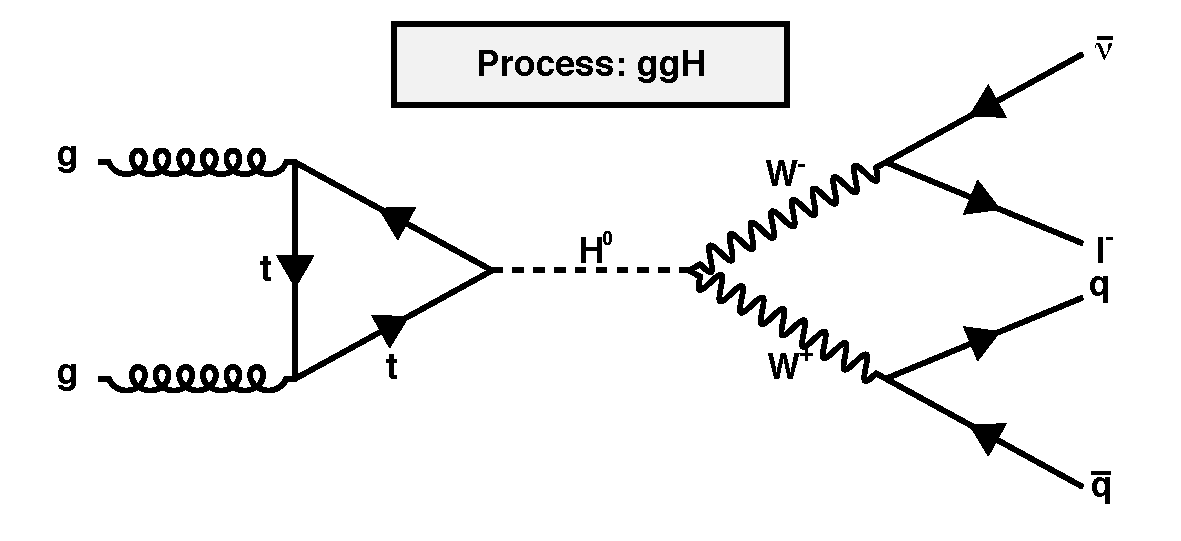
\includegraphics[width=0.5\textwidth]{\figpath/ggH_new.pdf}
			\end{center}
		}
		\only<2> {
			\begin{center}
				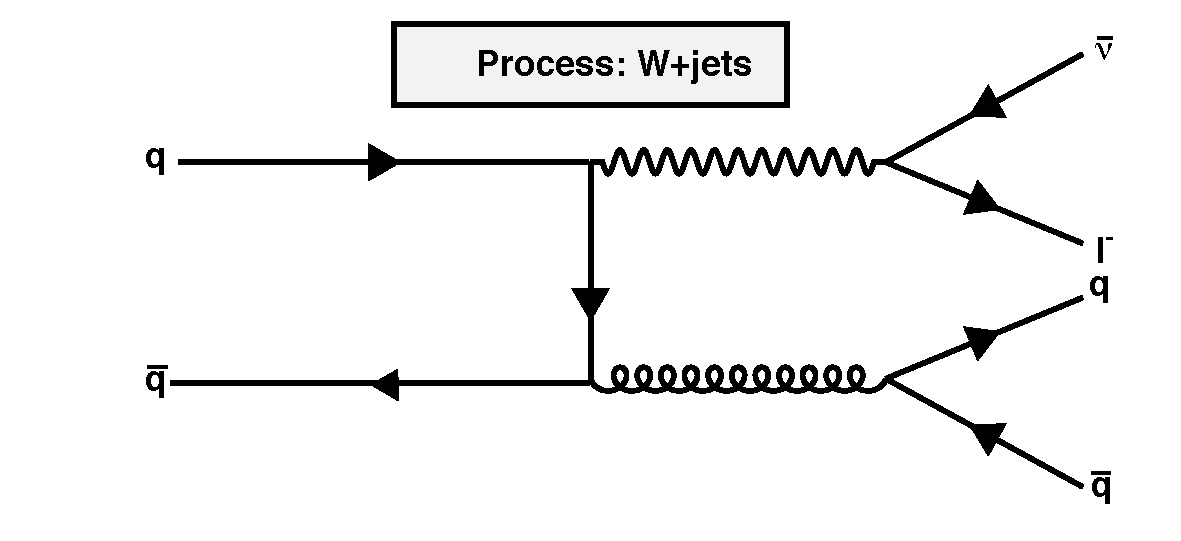
\includegraphics[width=0.5\textwidth]{\figpath/WJets1_new.pdf}
			\end{center}
		}
		\only<3-> {
		\begin{equation}\label{eq:MEM_probability}
%P_{sig}\left(x,m_{H}\right)=\frac{1}{N}\int_{y,q_{1},q_{2}}d\Phi\left(y\right)|M_{ggH}\left(y,m_{H}\right)|^{2}W\left(x,y\right)f_{pdf}\left(q_{1}\right)f_{pdf}\left(q_{2}\right)dq_{1}d1_{2}\\
{\color<8>{red}P_{i}}={\int}{\color<6>{red}T\left(\mathbf{X};\mathbf{Y}\right)}\frac{1}{\sigma_{i}}\sum_{flavor}\int_{V_{n}}{\color<4>{red}\mathcal{M}_{i}^{2}}\left(\mathbf{Y}\right)\frac{{\color<5>{red}f_{1}\left(q_{1},Q^{2}\right)f_{2}\left(q_{2},Q^{2}\right)}}{|\vec{q}_{1}|\cdot|\vec{q}_{2}|}{\color<7>{red}d\Phi_{n}\left(q_{1}+q_{2};y_{1},...,y_{n}\right)}d\mathbf{Y}
		\end{equation}
		\vspace*{-0.15cm}
		\begin{equation}\label<3>{eq:MEM_phaseSpace}
d\Phi_{n}\left(q_{1}+q_{2};y_{1},...,y_{n}\right)=\left(2\pi\right)^{4}\delta^{4}\left(q_{1}+q_{2}-\sum_{i=1}^{n}y_{i}\right)\prod_{i=1}^{n}\frac{d^{3}y_{i}}{\left(2\pi\right)^{3}2E_{i}}
		\end{equation}
		\vspace*{-0.15cm}
		\begin{itemize}
			\scriptsize
			\uncover<4->{\item $\mathcal{M}_{i}$ is the matrix element for the $2{\rightarrow}n$ process $i$}
			\uncover<5->{\item $f_{1}$ and $f_{2}$ are the PDF for the colliding partons $q_{1}$ and $q_{2}$ with beam energy fractions $x_{1}$ and $x_{2}$}
			\uncover<6->{\item $T\left(\vec{x},\vec{y}\right)$ is the transfer function, which maps the measured jet energies to the possible parton energies}
			\uncover<7->{\item $d\Phi$ (equation~\ref{eq:MEM_phaseSpace}) is the n-body phase space term}
			\uncover<8->{\item For each event we evaluate $P_{i}$ for 15 different processes}
		\end{itemize}
		}
	\end{block}
\end{frame}
%\againframe<2>{frame:MEM_formalism}
%\againframe<3>{frame:MEM_formalism}
%\againframe<4>{frame:MEM_formalism}
%\againframe<5>{frame:MEM_formalism}
%\againframe<6>{frame:MEM_formalism}
%\againframe<7>{frame:MEM_formalism}
%\againframe<8>{frame:MEM_formalism}

\begin{frame}
	\frametitle{Matrix Element Analysis}
	\framesubtitle{Evaluation}
	\vspace*{-0.24cm}
	\begin{block}{Monte Carlo Integration}
		\begin{itemize}
			\item Integration was performed using the \textbf{adaptive quadrature} method in the ROOT software package
			\begin{itemize}
				\item Based upon the CERNLIB RADMUL routine
			\end{itemize}
			\item The integral is computed over N-dimensional rectangular regions to an attempted, user-specified accuracy ($\epsilon$)
		\end{itemize}
		\begin{equation}
			I_{n}=\int_{a_{n}}^{b_{n}}\int_{a_{n-1}}^{b_{n-1}}\ldots\int_{a_{1}}^{b_{1}}f\left(x_{1},x_{2},\ldots,x_{n}\right)dx_{1}dx_{2}{\ldots}dx_{n}
		\end{equation}
		\vspace*{-0.40cm}
		\begin{itemize}
			\item The integration space is iteratively subdivided\\into $B_{i}$ regions
			\begin{itemize}
				\item A region is divided in half, along the axis\\most difficult to integrate, if the error\\within that region is the largest of all regions
				\item This stops when $\epsilon$ is reached
			\end{itemize}
			\item For each rectangular subregion there are\\$2^{n}+2n^{2}+2n+1$ function evaluations
		\end{itemize}
		\vspace*{-0.035cm}
		{\tiny A. van Doren and L. de Ridder, An adaptive algorithm for numerical integration over an n-dimensional cube, J. Comput. Appl. Math. 2 (1976) 207-217.}
	\end{block}
	\begin{textblock}{0.25}(0.68,0.540)
		\includegraphics[width=\textwidth]{\figpath/AdaptiveQuadratureRADMUL.png}
	\end{textblock}
\end{frame}

\begin{frame}
	\frametitle{Matrix Element Analysis}
	\framesubtitle{Computation \& Combination of Probability Densities}
	\vspace*{-0.24cm}

	\begin{block}{MEM Computation}
		\begin{itemize}
			\small
			\item The probabilities are calculated for a total of \textbf{62 processes/masses}
			\begin{itemize}
				\item \textbf{Computation Time}: $\sim12$ million CPU hours
			\end{itemize}
			\item The following 15 are the ones used in this analysis (all 3 dimensional integrations)
		\end{itemize}
		\vspace*{-0.3cm}
		\begin{columns}[T]
			\footnotesize
			\column{0.14\textwidth}
			\begin{itemize}
				\item {\color{red}$\cmsSymbolFace{W}\cmsSymbolFace{W}$}
				\item {\color{red}$\cmsSymbolFace{W}\cmsSymbolFace{Z}$}
				\item {\color{red}$\cmsSymbolFace{W}\cmsSymbolFace{Z}\cPqb\cPqb$}
				\item {\color{red}$\cmsSymbolFace{W}\cmsSymbolFace{L}\cPg$}
			\end{itemize}
			\column{0.27\textwidth}
			\begin{itemize}
				\item {\color{red}$\cmsSymbolFace{W}\cmsSymbolFace{L}\cPg$ (second order)}
				\item {\color{red}$\cmsSymbolFace{W}\cmsSymbolFace{L}\cmsSymbolFace{L}$}
				\item {\color{red}$\cmsSymbolFace{W}\cPg\cPg$}
				\item {\color{red}$\cmsSymbolFace{W}\cmsSymbolFace{L}\cPqb$}
			\end{itemize}
			\column{0.29\textwidth}
			\begin{itemize}
				\item {\color{red}$\cmsSymbolFace{W}\cPqb\cPqb$}
				\item {\color{red}ZLight}
				\item {\color{red}Single Top \cPqs-channel}
				\item {\color{red}Single Top \cPqt-channel}
			\end{itemize}
			\column{0.30\textwidth}
			\begin{itemize}
				\item {\color{red}QCD}
				\item {\color{red}ggH (\MH=125\gev)}
				\item {\color{red}WH (\MH=125\gev)}
			\end{itemize}
		\end{columns}
	\end{block}
	\vspace*{-0.24cm}
	\begin{block}{We still needed to combine the 15 MEs into some discriminator}
	 	\begin{itemize}
	 		\item Could have followed the CDF Single Top analysis or the CMS $\PH{\rightarrow}\ZZ{\rightarrow}4\ell$ analysis in making use of the Neyman-Pearson lemma to form a ratio of likelihoods
	 		%\begin{itemize}
	 		%	\item In CMS this is called a Matrix Element Likelihood Analysis (MELA)
	 		%\end{itemize}
	 		\item We found this methodology to be inferior to using a \textbf{Boosted Decision Tree (BDT)} classifier
	 		\begin{itemize}
	 			\item This gives a typically shallow networked (BDT) the ability to create a non-linear discriminant function because the inputs are already non-linear variables
	 		\end{itemize}
	 	\end{itemize}
	\end{block}
\end{frame}

\begin{frame}<1>[label=frame:MEM_computation_combination]
	\frametitle{Matrix Element Analysis}
	\framesubtitle{ME BDT Results}
	\vspace*{-0.24cm}
	\begin{textblock}{0.96}(0.0175,0.14)
		\begin{block}{}
			\begin{itemize}
				\item BDT discriminant computed for individual jet bins
				\begin{itemize}
					\item {\color{blue}Blue: Signal}
					\item {\color{red}Red: Background}
				\end{itemize}
			\end{itemize}
		\end{block}
	\end{textblock}
	\begin{textblock}{0.96}(0.0175,0.33)
		\begin{alertblock}{BDT Discriminants}
			\centering
			\includegraphics[width=0.33\textwidth]{\figpath/MVA/2015_07_17_TMVA_output_jets2_eq0tag_both_HToWW_WJets_allEvtProbs_0KinVar/mva_BDT.pdf}%
			\includegraphics[width=0.33\textwidth]{\figpath/MVA/2015_07_17_TMVA_output_jets3_eq0tag_both_HToWW_WJets_allEvtProbs_0KinVar/mva_BDT.pdf}%
			\includegraphics[width=0.33\textwidth]{\figpath/MVA/2015_07_17_TMVA_output_jets4_eq0tag_both_HToWW_WJets_allEvtProbs_0KinVar/mva_BDT.pdf}%
		\end{alertblock}
	\end{textblock}
	\begin{textblock}{0.15}(0.24,0.53){\color{red}{2 Jets}}\end{textblock}
	\begin{textblock}{0.15}(0.56,0.53){\color{red}{3 Jets}}\end{textblock}
	\begin{textblock}{0.15}(0.88,0.53){\color{red}{$\geq$4 Jets}}\end{textblock}
	\begin{textblock}{0.96}(0.0175,0.76)
		\begin{block}{}
			\begin{itemize}
				\item Some discrimination between signal and background
				\begin{itemize}
					\item Tough analysis given the similar kinematics of signal and background
				\end{itemize}
				\item ME is LO only and permutations of jets and partons degrades discrimination
			\end{itemize}
		\end{block}
	\end{textblock}
\end{frame}